% Chapter 1
\chapter{مقدمه}

\section{شناخت موضوع}
در سال‌های اخیر، به دلیل پیشرفت‌های سریع فناوری و دسترسی آسان به اینترنت، بسیاری از دستگاه‌ها به اینترنت متصل شده‌اند. این پدیده که به اینترنت اشیا%
\LTRfootnote{Internet of Things}
معروف است، شامل انواع دستگاه‌ها از جمله دستگاه‌های پوشیدنی%
\LTRfootnote{Wearable Devices}%
، خودروهای خودران، خانه‌های هوشمند%
\LTRfootnote{Smart Homes}
و به ویژه تلفن‌های هوشمند%
\LTRfootnote{Smart Phones}
می‌شود. این دستگاه‌ها به‌طور چشمگیری زندگی روزمره انسان‌ها را دگرگون کرده‌اند. استفاده از این سیستم‌ها همگی باعث تولید حجم قابل توجهی داده در طول روز می‌شوند که شرکت‌های بزرگ فناوری از این داده‌ها بهره برده و با استفاده از آن‌ها اقدام به ارائه انواع سرویس به کاربران خود می‌نمایند. همچنین این روند سبب ظهور فناوری هوش مصنوعی و موارد مرتبط با آن شده است.

با پیشرفت علم هوش مصنوعی و استفاده گسترده از روش‌های یادگیری ماشین، امکان بهره‌برداری بهینه از حجم عظیم داده‌های تولید شده فراهم گردیده است. این داده‌ها می‌توانند برای اجرای الگوریتم‌های مختلف به منظور دستیابی به اهداف متنوع به کار گرفته شوند. روش‌های متعددی برای مدیریت و اجرای این الگوریتم‌های یادگیری وجود دارد که در ادامه به توضیح هر یک پرداخته خواهد شد.


\subsection{
	یادگیری متمرکز%
	\LTRfootnote{Centralized Learning}
}
در روش یادگیری متمرکز که در بسیاری از سیستم‌های امروزی به کار می‌رود، تمامی گره‌ها%
\LTRfootnote{Nodes}
اطلاعات خود را به‌طور کامل به یک سرویس‌دهنده ابری%
\LTRfootnote{Cloud Server}
ارسال می‌کنند و سرویس‌دهنده با دسترسی به تمامی داده‌ها، الگوریتم‌های مورد نیاز را اجرا می‌کند. این روش به دلیل تمرکز داده‌ها در یک مکان مرکزی، امکان اجرای دقیق و هماهنگ الگوریتم‌ها را فراهم می‌کند، اما وابستگی به سرویس‌دهنده مرکزی می‌تواند منجر به مشکلات امنیتی و چالش‌های مقیاس‌پذیری شود
\cite{elbir2022family}.
این روش در شکل
\ref{centralized_learning}
به تصویر کشیده شده است.


\subsection{
	یادگیری غیرمتمرکز%
	\LTRfootnote{Decentralized Learning}
}
در روش یادگیری غیرمتمرکز، هر گره به‌طور مستقل الگوریتم‌های مورد نیاز خود را اجرا کرده و پس از چند مرحله، اطلاعات به‌روزرسانی‌شده را با گره‌های همسایه به اشتراک می‌گذارد. این فرآیند تا زمان دستیابی به همگرایی کامل بین گره‌ها ادامه پیدا می‌کند. این روش با بهره‌گیری از استقلال گره‌ها، باعث افزایش مقیاس‌پذیری و مقاومت در برابر خرابی‌های سیستم می‌شود، اما در عین حال، ممکن است به تبادل مکرر اطلاعات و تأخیر در دستیابی به همگرایی منجر شود
\cite{zhou2019edge}.
این روش در شکل
\ref{decentralized_learning}
به نمایش در آمده است.

\subsection{
	یادگیری توزیع شده%
	\LTRfootnote{Distributed Learning}
}
در روش یادگیری توزیع‌شده، یک هسته مرکزی مدیریت کل سیستم و داده‌ها را بر عهده دارد، اما برای کاهش فشار پردازشی، این بار را بین گره‌های موجود توزیع می‌کند. این تقسیم بار پردازشی منجر به سرعت و کارایی بیشتر در فرآیند آموزش می‌شود و امکان استفاده همزمان از منابع متنوع برای تحلیل داده‌های بزرگ را فراهم می‌آورد. با این حال، وابستگی به هسته مرکزی ممکن است نقطه‌ضعفی باشد که می‌تواند به بروز مشکلاتی در صورت خرابی یا اختلال در عملکرد آن منجر شود.
این روش در شکل
\ref{distributed_learning}
نشان داده شده است.


\begin{figure}[t!]
	\centering
	\subfigure[
	یادگیری متمرکز
	\cite{zhou2019edge}
	]{
		\label{centralized_learning}
		\includegraphics*[width=.31\textwidth]{images/chap1/centralized_learning.png}
	}
	\hspace{0.5mm}
	\subfigure[
	یادگیری غیرمتمرکز
	\cite{zhou2019edge}
	]{
		\label{decentralized_learning}
		\includegraphics*[width=.31\textwidth]{images/chap1/decentralized_learning.png}
	}
	\hspace{0.5mm}
	\subfigure[یادگیری توزیع‌شده]{
		\label{distributed_learning}
		\includegraphics*[width=.31\textwidth]{images/chap1/distributed_learning.png}
	}
	\caption{انواع روش‌های یادگیری.}
	\label{learning_methods}
\end{figure}



\section{
	یادگیری فدرال%
	\LTRfootnote{Federated Learning}
}\label{federated_learning_section}
سیستم‌های متمرکز تا پیش از این بیشتر نیازها را برطرف می‌کردند، اما در دنیای امروزی و با افزایش تعداد دستگاه‌های متصل، چالش‌های جدیدی مطرح شده است. هزینه‌های بالای ناشی از انتقال حجم زیاد داده‌ها از یک جهت، و افزایش نگرانی‌ها درباره امنیت اطلاعات حساس و شخصی از جهت دیگر، محققان را به سمت استفاده از الگوریتم‌های غیرمتمرکز و توزیع‌شده در حوزه یادگیری ماشین سوق داده است. یکی از جدیدترین زیرمجموعه‌های مهم و پرکاربرد روش‌های یادگیری توزیع‌شده، یادگیری فدرال است که بسیار مورد توجه قرار گرفته است.


در روش یادگیری فدرال، برخلاف رویکردهای متمرکز یادگیری ماشین، تجزیه و تحلیل داده‌ها به دستگاه‌های لبه%
\LTRfootnote{Edge Devices}
یا کاربران%
\LTRfootnote{Clients}
منتقل می‌شوند
\cite{ma2022state}.
این روش، به عنوان یک جایگزین مطلوب برای مدل‌سازی داده‌ها در محیط‌هایی با تعداد زیادی کاربر معرفی شده است. در این چارچوب، به‌جای انتقال داده‌های اصلی، پارامترهای مدل‌های محلی در هر مرحله از فرآیند آموزش به سمت سرور منتقل می‌شوند، که این امر زمینه‌ساز بهبود امنیت و کاهش هزینه‌های ارتباطی می‌باشد.
در شکل
\ref{federated_learning}
این معماری به نمایش گذاشته شده است.


 \begin{figure}[t!]
	\centering
	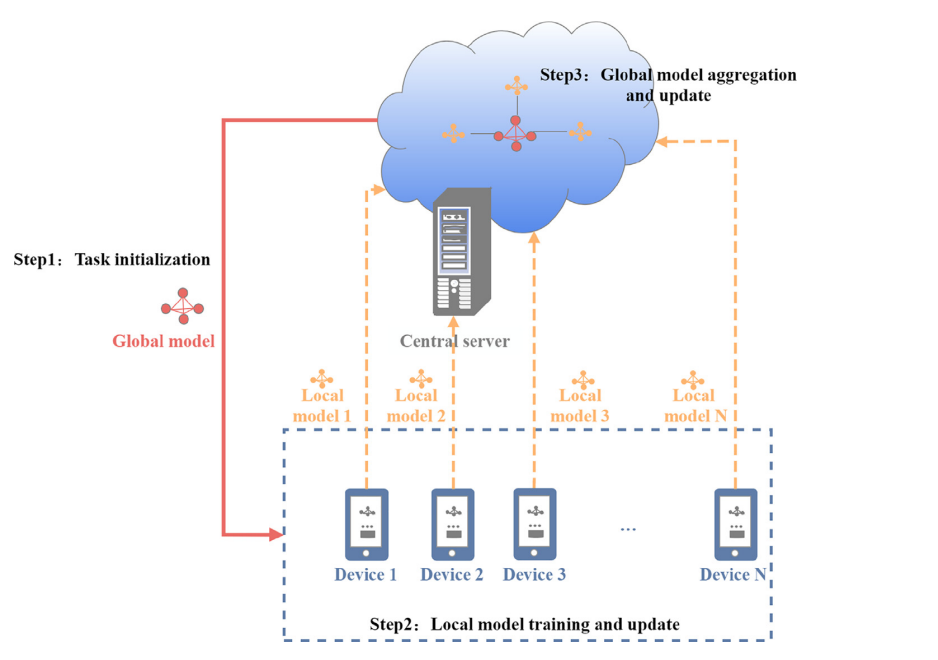
\includegraphics[scale=0.595]{images/chap1/federated_learning.png}%
	\caption{%
		یادگیری فدرال 
		\cite{ma2022state}%
		.
	}
	\label{federated_learning}
	\centering
\end{figure}

سرور در حقیقت نقش رهبری را ایفا می‌کند و با توجه به نوع داده‌ها، یک مدل شبکه عصبی%
\LTRfootnote{Neural Network}
ایجاد کرده و آن را به سمت کاربران ارسال می‌کند. در ادامه کاربران با توجه به داده‌های خود شبکه را آموزش می‌دهند و بعد از چند بار تکرار به‌صورت محلی، وزن‌های به‌روزرسانی شده را به سمت سرور بر می‌گردانند. همان‌طور که در شکل
\ref{federated_learning}
مشاهده می‌شود، داده‌ها همگی در سمت کاربران قرار گرفته‌اند و به سمت سرور ارسال نمی‌شوند. عدم اجبار در به اشتراک گذاشتن اطلاعات گره‌ها در یادگیری فدرال، کمک شایانی به حفظ حریم شخصی کاربران می‌کند
\cite{smith2017federated}.



\section{تاریخچه یادگیری فدرال}


در اوایل فصل بهار سال 2017، محققان گوگل
\lr{(Google)}
برای اولین بار موضوع یادگیری فدرال را در یک مطلب کوتاه در وبلاگ هوش مصنوعی خود معرفی کردند. این مطلب با عنوان «یادگیری فدرال: یادگیری ماشین اشتراکی، بدون نیاز به آموزش متمرکز داده‌ها» منتشر شد
\cite{brendan2017federated}.
در این نوشته، به‌طور مختصر از
\lr{Google Keyboard}
یا به اختصار
\lr{Gboard}
صحبت شد که با بهره‌گیری از یادگیری فدرال، قابلیت پیش‌بینی و پیشنهاد لغت بعدی به کاربر را دارد. با استفاده از یادگیری فدرال، دیگر نیازی به ارسال داده‌های کاربران به سرور نبود و مدل به ‌صورت محلی به‌روزرسانی می‌شد.

این روش با استفاده از اطلاعات فراوان ذخیره شده در دستگاه‌ها، خدمات بهتری را ارائه می‌دهد، بدون این که داده‌های حساس به سرور ارسال شوند و حریم شخصی کاربران به خطر بیفتد. در شکل
\ref{gboard}%
، نحوه استفاده از یادگیری فدرال در این برنامه به نمایش درآمده است.


 \begin{figure}[t!]
	\centering
	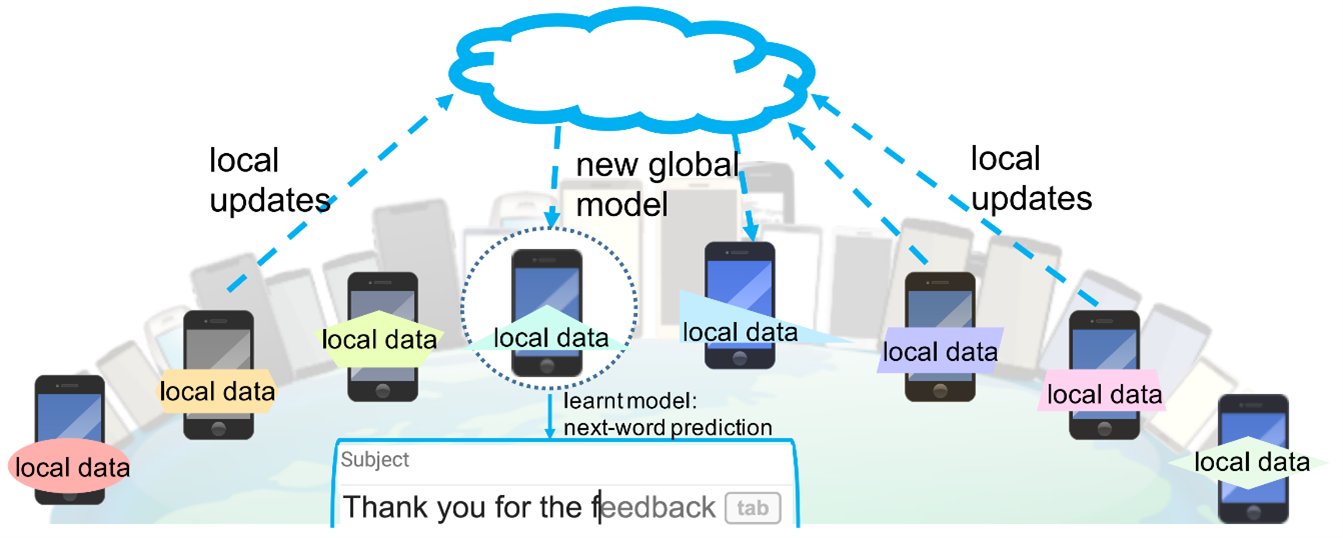
\includegraphics[scale=1]{images/chap1/gboard.png}%
	\caption{%
استفاده از یادگیری فدرال برای پیش‌بینی کلمه بعدی در
\lr{Gboard}
		\cite{li2020federated}%
		.
	}
	\label{gboard}
	\centering
\end{figure}



\section{کاربرد یادگیری فدرال}
سامانه‌های متمرکز سنتی که تنها مسئول جمع‌آوری، پایش و کنترل شرایط به‌صورت محلی بودند، اکنون جای خود را به دستگاه‌های هوشمندی داده‌اند که قابلیت پردازش و برنامه‌ریزی داده‌ها را در سطح سیار و سیستمی دارند. علاوه بر این، گسترش ارتباطات مبتنی‌بر اینترنت، امکان انتقال و تبادل داده‌ها بین سیستم‌های مختلف را فراهم کرده است. این تحولات منجر به کاهش نیاز به تصمیم‌گیری متمرکز و توسعه سیستم‌های کنترل و پایش پیشرفته شده است. این ویژگی‌ها، همراه با حجم روزافزون داده‌ها، یادگیری فدرال را به یکی از بهترین روش‌ها برای توسعه سیستم‌های هوشمند تبدیل کرده است
\cite{mahtab2022algorithm}.
در ادامه، سه نمونه از کاربردهای یادگیری فدرال شرح داده خواهد شد.


\subsection{
	یادگیری فدرال در شهر هوشمند%
	\LTRfootnote{Smart City}
}
در یک شهر هوشمند، اطلاعات جمع‌آوری شده از حسگرهای مختلف مانند داده‌های ترافیک، مصرف انرژی، پسماند شهری و رویدادهای امنیتی، ارزش بالایی دارند و به عنوان منبعی کلیدی برای بهبود عملکرد شهر هوشمند و ارتقای کیفیت زندگی شهروندان محسوب می‌شوند. اما در کنار این مزایا، حفظ حریم شخصی و امنیت اطلاعات شهروندان نیز از اهمیت بالایی برخوردار است. در این‌جا یادگیری فدرال به عنوان یک رویکرد نوین که مبتنی‌بر حفظ حریم شخصی است، به کار گرفته می‌شود.

اگرچه در یک شهر هوشمند، سازمان‌های مختلف هر کدام اطلاعات خاص خود را دارند، اما با تجمیع این اطلاعات می‌توان مدیریت بهتری انجام داد. یادگیری فدرال با حفظ حریم شخصی کاربران، این امکان را فراهم می‌کند که سازمان‌ها بدون نیاز به اشتراک‌گذاری داده‌های حساس خود با یکدیگر، از تمامی داده‌های موجود بهره‌برداری کنند و مدل‌های هوش مصنوعی و الگوریتم‌های بهبود عملکرد شهر هوشمند را توسعه دهند. به عنوان مثال، با استفاده از یادگیری فدرال می‌توان بهبود مدیریت ترافیک، بهینه‌سازی مصرف انرژی، کاهش آلودگی هوا و افزایش امنیت شهری را تحقق بخشید، در حالی که حریم شخصی شهروندان به بهترین شکل حفظ می‌شود.


\subsection{یادگیری فدرال در بیمارستان}
در یک بیمارستان، اطلاعات پزشکی دارای طبقه‌بندی حساس و مهم هستند و باید به‌صورت محرمانه نگهداری شوند. با این حال، بهره‌برداری از این داده‌ها برای ارتقاء خدمات بهداشتی و درمانی بسیار ارزشمند است. در این شرایط، یادگیری فدرال می‌تواند نقش مهمی ایفا کند. با استفاده از روش‌های یادگیری فدرال، بیمارستان‌ها می‌توانند از داده‌های پزشکی بیماران خود برای توسعه مدل‌هایی استفاده کنند که به بهبود خدمات، ارتقاء روش‌های تشخیص و درمان بیماری‌ها و افزایش بهره‌وری پزشکان کمک می‌کنند، بدون این که نیاز باشد این داده‌ها به‌طور مستقیم به یک مرکز جمع‌آوری اطلاعات ارسال شوند.

به عبارت دیگر، یادگیری فدرال این امکان را فراهم می‌کند که مدل‌های هوش مصنوعی روی داده‌های محلی بیماران در هر بیمارستان آموزش ببینند و بیماری‌ها را شناسایی و تشخیص دهند. این فرایند به بهبود درمان‌ها کمک می‌کند، بدون این که اطلاعات حساس بیماران به بیرون درز کند و امنیت آن‌ها حفظ می‌شود. در شکل
\ref{hospital}
شمای کلی استفاده از یادگیری فدرال در بیمارستان‌ها به نمایش در آمده است.


\begin{figure}[b!]
	\centering
	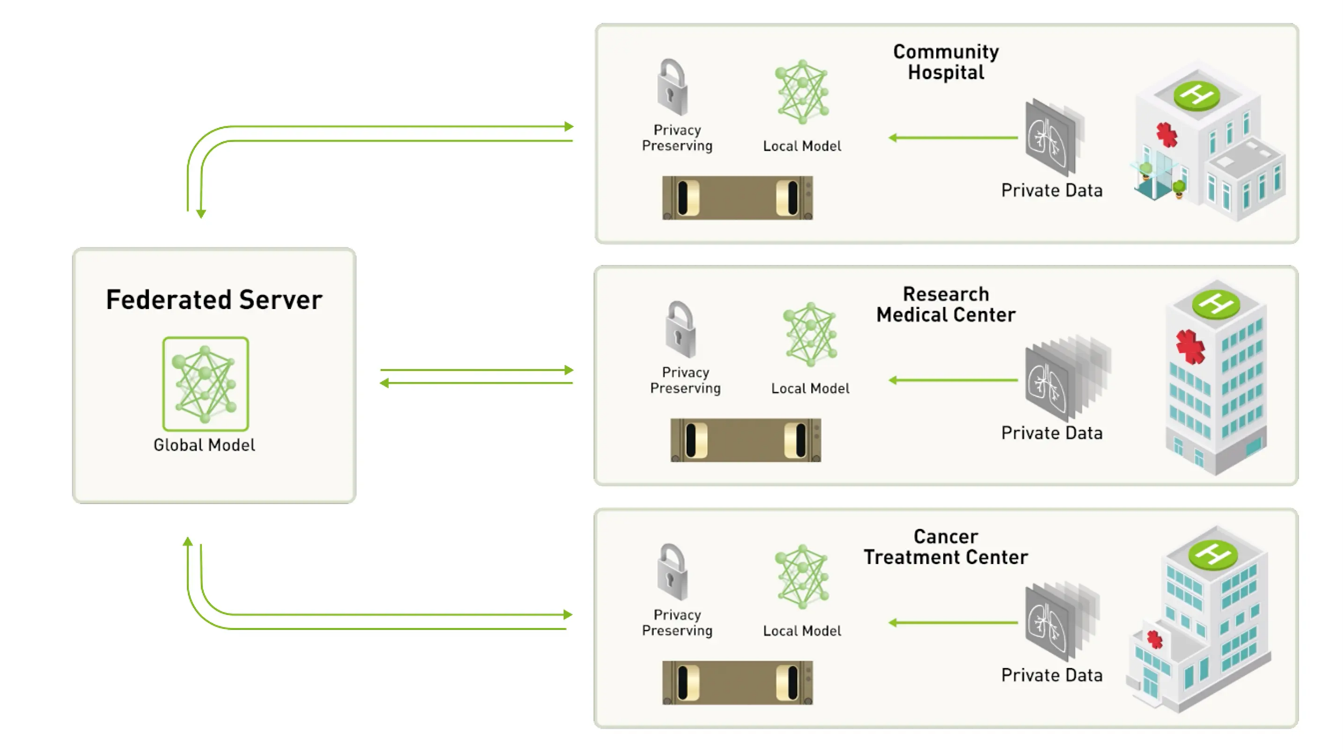
\includegraphics[scale=1]{images/chap1/hospital.png}%
	\caption{%
		کاربرد یادگیری فدرال در بیمارستان
		\cite{rieke2019what}%
		.
	}
	\label{hospital}
	\centering
\end{figure}



\subsection{
	یادگیری فدرال در فروشگاه برنامه‌های کاربردی%
	\LTRfootnote{App Store}
	تلفن‌همراه
}
یک فروشگاه مجازی برنامه‌های کاربردی تلفن‌همراه را در نظر بگیرید که به کاربران امکان دریافت و نصب برنامه‌های مختلف را می‌دهد. این فروشگاه می‌خواهد با استفاده از داده‌های کاربران خود، الگوریتمی را توسعه دهد که بتواند به‌طور دقیق‌تری برنامه‌های مورد علاقه کاربران را به آن‌ها پیشنهاد دهد. اگر این فروشگاه از روش‌های متمرکز استفاده کند، باید داده‌های حساس و شخصی کاربران را جمع‌آوری و تحلیل کند که این موضوع می‌تواند نگرانی‌های جدی در مورد حریم شخصی کاربران ایجاد کند و غیرعملی باشد.

در حالی که با استفاده از یادگیری فدرال، این فروشگاه می‌تواند الگوریتم خود را بر روی داده‌های محلی هر کاربر اجرا کند. به این ترتیب، هیچ داده حساسی به یک مرکز جمع‌آوری داده‌ها ارسال نمی‌شود و حریم شخصی کاربران حفظ می‌گردد. به عنوان مثال، اگر یک کاربر به برنامه‌های موسیقی علاقه‌مند باشد، الگوریتم محلی در تلفن هوشمند او می‌تواند این الگو را شناسایی کند و پیشنهادهای مربوط به برنامه‌های موسیقی را ارائه دهد، بدون این که نیاز به ارسال داده‌های شخصی و حساس او به سرور فروشگاه باشد.


\section{انگیزه و هدف پژوهش}

در یادگیری فدرال، توزیع داده‌ها و پردازش آن‌ها در سیستم‌های مختلف و مستقل، چالش‌های زیادی را ایجاد می‌کند. یکی از این چالش‌ها، تفاوت‌های سیستمی و تنوع داده‌ها بین کاربران مختلف است که فرآیند آموزش مدل‌ها را پیچیده می‌کند. بنابراین، برای بهبود کارایی مدل‌های فدرال و مقابله با این مشکلات، نیاز به روش‌های خلاقانه و مؤثر احساس می‌شود.

همان‌گونه که بیان شد، یکی از چالش‌های اصلی، مواجهه با داده‌های بسیار گوناگون و متفاوتی است که در بین کاربران مختلف پراکنده شده‌اند. این پراکندگی منجر به کندی فرایند همگرایی مدل‌های یادگیری می‌شود. به‌طور معمول، داده‌های موجود در یک دستگاه با داده‌های دستگاه‌های دیگر تفاوت‌های قابل توجهی دارند و این تفاوت‌ها باعث می‌شود تا مدل سراسری نتواند به‌سرعت به یک دقت مطلوب دست یابد. این مشکل باعث شده است تا پژوهشگران به دنبال راهکارهایی باشند که بتوانند این فرایند را تسریع کرده و مدل سراسری را به دقت بالاتری برسانند
\cite{li2020federated}.

یکی از روش‌های پیشنهادی برای حل این مشکل، جابه‌جایی وزن‌های شبکه‌های عصبی بین کاربران نهایی در طول فرایند یادگیری است
\cite{chiu2020semisupervised}.
این جابه‌جایی مدل‌ها بین کاربران، می‌تواند به تغییر وزن‌ها منجر شده و به مدل‌ها کمک کند تا با داده‌های متفاوتی آشنا شوند.
به عبارت دیگر، این روش از طریق فراهم کردن امکان آشنایی با داده‌های جدید می‌تواند همگرایی مدل سراسری را بهبود بخشد و مدل را به سمت مقادیر بهتری هدایت کند.

با این حال، در روش‌های قبلی، این جابه‌جایی‌ها به‌طور تصادفی انجام می‌شدند. این تصادفی بودن ممکن است باعث شود که مدل‌ها با داده‌هایی مواجه شوند که قبلاً با آن‌ها آشنا بوده‌اند یا تغییرات ایجاد شده در وزن‌ها نتوانند بهبود قابل‌توجهی در دقت مدل ایجاد کنند. بنابراین، این سوال مطرح می‌شود که آیا می‌توان به جای استفاده از جابه‌جایی تصادفی، این فرایند را به‌صورت هوشمندانه‌تری انجام داد، به این صورت که با استفاده از معیارهای مشخص، مدل‌هایی که بیشترین تفاوت را با یکدیگر دارند شناسایی و با هم مبادله شوند.

پژوهش حاضر بر آن است که پاسخ این پرسش را مورد بررسی قرار داده و روشی مناسب در این رابطه ارائه نماید. در روش پیشنهادی سعی خواهد شد، دو مدلی که کمترین میزان شباهت را با یکدیگر دارند، جابه‌جا شوند. این رویکرد بر این اساس استوار است که مدل‌هایی که شباهت زیادی به یکدیگر دارند، نشان‌دهنده این هستند که کاربران نهایی آن‌ها داده‌های نسبتاً مشابهی دارند. در مقابل، مدل‌هایی که شباهت کمتری با یکدیگر دارند، در واقع با داده‌های متفاوت‌تری آموزش دیده‌اند.
جابه‌جایی مدل‌هایی که داده‌های متفاوتی را مشاهده کرده‌اند، می‌تواند به این معنا باشد که این مدل‌ها می‌توانند با داده‌های جدیدی آشنا شوند که پیش‌تر با آن‌ها روبه‌رو نشده بودند. این آشنایی با داده‌های جدید می‌تواند به شبکه عصبی سراسری کمک کند تا بهتر با داده‌های مختلفی که توسط کاربران گوناگون تولید می‌شوند، تطابق پیدا کند. در نتیجه، شبکه عصبی سراسری می‌تواند سریع‌تر و با دقت بیشتری به همگرایی نهایی برسد.

علاوه بر هدف اصلی که در بالا به آن اشاره شد، حفظ حریم شخصی نیز مسئله‌ای است که باید در نظر گرفته شود.
در پژوهش‌های پیشین، مدل‌ها به‌صورت مستقیم و بدون واسطه بین کاربران جابه‌جا می‌شدند. اما در روش پیشنهادی این تحقیق، جابه‌جایی مدل‌ها با واسطه سرور صورت می‌گیرد که این رویکرد می‌تواند به بهبود حفظ حریم شخصی کاربران کمک کند. بنابراین می‌توان گفت که اگرچه تمرکز اصلی این پژوهش بر بهبود عملکرد مدل نهایی از نظر دقت است، اما تلاش‌هایی نیز برای ارتقای سطح حریم شخصی صورت گرفته است.

در نتیجه‌ می‌توان این‌طور بیان کرد که این پژوهش روش هوشمندانه‌ای برای جابه‌جایی مدل‌ها بر پایه شباهت پیشنهاد می‌دهد که می‌تواند به عنوان راهکاری مؤثر در تسریع همگرایی یادگیری فدرال مورد استفاده قرار گیرد. این روش نه تنها باعث بهبود کیفیت مدل سراسری می‌شود، بلکه کارایی آن را در برخورد با داده‌های مختلف کاربران نیز افزایش می‌دهد.


\section{مروری بر روند ارائه مطالب پایان‌نامه}

در فصل دوم، ابتدا مفاهیم پایه‌ای در یادگیری ماشین و یادگیری عمیق توضیح داده شده و ارتباط آن‌ها با یادگیری فدرال بررسی می‌شود. همچنین چارچوب ریاضی مربوط به یادگیری فدرال ارائه می‌گردد. پس از آن، چالش‌های موجود در این حوزه تحلیل شده و دیدگاه‌های مختلف مقالات در این زمینه مرور می‌شوند. در پایان، راهکارهای اساسی ارائه شده برای حل این چالش‌ها مورد بحث قرار می‌گیرند.

فصل سوم به بررسی جامع پیشینه روش‌های حل مشکل توزیع متفاوت و گوناگون داده‌ها میان کاربران مختلف در شبکه اختصاص دارد. این بررسی از منظر داده، مدل، چارچوب و الگوریتم انجام می‌شود.

در فصل چهارم، روش جابه‌جایی مدل‌ها معرفی شده و نحوه جابه‌جایی تصادفی و نیز روش جابه‌جایی بر پایه شباهت بررسی می‌گردند. سپس تأثیر این جابه‌جایی‌ها بر ترافیک شبکه و حریم شخصی تحلیل می‌شود. در ادامه معیارهای شباهت و پایداری آن‌ها نیز مورد بررسی قرار گرفته و تعدادی شاخص برای سنجش شباهت معرفی می‌گردد. در نهایت، روش‌های مختلف برای تعیین کاربران نهایی جهت جابه‌جایی مدل‌ها توضیح داده می‌شود.

در فصل پنجم، ابتدا به توضیح مدل‌های شبکه عصبی که در این پژوهش پیاده‌سازی شده‌اند، پرداخته می‌شود. سپس، انواع مجموعه داده‌های مورد استفاده معرفی و روش جابه‌جایی بر پایه شباهت با سایر روش‌های مرجع در این مجموعه داده‌ها مقایسه می‌شوند. علاوه بر این، تاثیر روش‌های مختلف جابه‌جایی، تغییر تعداد کاربران و تاثیر تعداد دورها نیز به‌طور دقیق تحلیل خواهند شد.
در پایان، فصل ششم به نتیجه‌گیری کلی و ارائه پیشنهادهایی برای ادامه پژوهش اختصاص خواهد داشت.